\documentclass[11pt]{article}

    \usepackage[breakable]{tcolorbox}
    \usepackage{parskip} % Stop auto-indenting (to mimic markdown behaviour)
    

    % Basic figure setup, for now with no caption control since it's done
    % automatically by Pandoc (which extracts ![](path) syntax from Markdown).
    \usepackage{graphicx}
    \graphicspath{{./images/}}

    % Maintain compatibility with old templates. Remove in nbconvert 6.0
    \let\Oldincludegraphics\includegraphics
    % Ensure that by default, figures have no caption (until we provide a
    % proper Figure object with a Caption API and a way to capture that
    % in the conversion process - todo).
    \usepackage{caption}
    \DeclareCaptionFormat{nocaption}{}
    \captionsetup{format=nocaption,aboveskip=0pt,belowskip=0pt}

    \usepackage{float}
    \floatplacement{figure}{H} % forces figures to be placed at the correct location
    \usepackage{xcolor} % Allow colors to be defined
    \usepackage{enumerate} % Needed for markdown enumerations to work
    \usepackage{geometry} % Used to adjust the document margins
    \usepackage{amsmath} % Equations
    \usepackage{amssymb} % Equations
    \usepackage{textcomp} % defines textquotesingle
    % Hack from http://tex.stackexchange.com/a/47451/13684:
    \AtBeginDocument{%
        \def\PYZsq{\textquotesingle}% Upright quotes in Pygmentized code
    }
    \usepackage{upquote} % Upright quotes for verbatim code
    \usepackage{eurosym} % defines \euro

    \usepackage{iftex}
	\usepackage[utf8]{inputenc}
    \usepackage[T1]{fontenc}

    \usepackage{fancyvrb} % verbatim replacement that allows latex
    \usepackage{grffile} % extends the file name processing of package graphics
                         % to support a larger range
    \makeatletter % fix for old versions of grffile with XeLaTeX
    \@ifpackagelater{grffile}{2019/11/01}
    {
      % Do nothing on new versions
    }
    {
      \def\Gread@@xetex#1{%
        \IfFileExists{"\Gin@base".bb}%
        {\Gread@eps{\Gin@base.bb}}%
        {\Gread@@xetex@aux#1}%
      }
    }
    \makeatother
    \usepackage[Export]{adjustbox} % Used to constrain images to a maximum size
    \adjustboxset{max size={0.9\linewidth}{0.9\paperheight}}

    % The hyperref package gives us a pdf with properly built
    % internal navigation ('pdf bookmarks' for the table of contents,
    % internal cross-reference links, web links for URLs, etc.)
    \usepackage{hyperref}
    % The default LaTeX title has an obnoxious amount of whitespace. By default,
    % titling removes some of it. It also provides customization options.
    \usepackage{titling}
    \usepackage{longtable} % longtable support required by pandoc >1.10
    \usepackage{booktabs}  % table support for pandoc > 1.12.2
    \usepackage{array}     % table support for pandoc >= 2.11.3
    \usepackage{calc}      % table minipage width calculation for pandoc >= 2.11.1
    \usepackage[inline]{enumitem} % IRkernel/repr support (it uses the enumerate* environment)
    \usepackage[normalem]{ulem} % ulem is needed to support strikethroughs (\sout)
                                % normalem makes italics be italics, not underlines
    \usepackage{mathrsfs}
    

    
    % Colors for the hyperref package
    \definecolor{urlcolor}{rgb}{0,.145,.698}
    \definecolor{linkcolor}{rgb}{.71,0.21,0.01}
    \definecolor{citecolor}{rgb}{.12,.54,.11}

    % ANSI colors
    \definecolor{ansi-black}{HTML}{3E424D}
    \definecolor{ansi-black-intense}{HTML}{282C36}
    \definecolor{ansi-red}{HTML}{E75C58}
    \definecolor{ansi-red-intense}{HTML}{B22B31}
    \definecolor{ansi-green}{HTML}{00A250}
    \definecolor{ansi-green-intense}{HTML}{007427}
    \definecolor{ansi-yellow}{HTML}{DDB62B}
    \definecolor{ansi-yellow-intense}{HTML}{B27D12}
    \definecolor{ansi-blue}{HTML}{208FFB}
    \definecolor{ansi-blue-intense}{HTML}{0065CA}
    \definecolor{ansi-magenta}{HTML}{D160C4}
    \definecolor{ansi-magenta-intense}{HTML}{A03196}
    \definecolor{ansi-cyan}{HTML}{60C6C8}
    \definecolor{ansi-cyan-intense}{HTML}{258F8F}
    \definecolor{ansi-white}{HTML}{C5C1B4}
    \definecolor{ansi-white-intense}{HTML}{A1A6B2}
    \definecolor{ansi-default-inverse-fg}{HTML}{FFFFFF}
    \definecolor{ansi-default-inverse-bg}{HTML}{000000}

    % common color for the border for error outputs.
    \definecolor{outerrorbackground}{HTML}{FFDFDF}

    % commands and environments needed by pandoc snippets
    % extracted from the output of `pandoc -s`
    \providecommand{\tightlist}{%
      \setlength{\itemsep}{0pt}\setlength{\parskip}{0pt}}
    \DefineVerbatimEnvironment{Highlighting}{Verbatim}{commandchars=\\\{\}}
    % Add ',fontsize=\small' for more characters per line
    \newenvironment{Shaded}{}{}
    \newcommand{\KeywordTok}[1]{\textcolor[rgb]{0.00,0.44,0.13}{\textbf{{#1}}}}
    \newcommand{\DataTypeTok}[1]{\textcolor[rgb]{0.56,0.13,0.00}{{#1}}}
    \newcommand{\DecValTok}[1]{\textcolor[rgb]{0.25,0.63,0.44}{{#1}}}
    \newcommand{\BaseNTok}[1]{\textcolor[rgb]{0.25,0.63,0.44}{{#1}}}
    \newcommand{\FloatTok}[1]{\textcolor[rgb]{0.25,0.63,0.44}{{#1}}}
    \newcommand{\CharTok}[1]{\textcolor[rgb]{0.25,0.44,0.63}{{#1}}}
    \newcommand{\StringTok}[1]{\textcolor[rgb]{0.25,0.44,0.63}{{#1}}}
    \newcommand{\CommentTok}[1]{\textcolor[rgb]{0.38,0.63,0.69}{\textit{{#1}}}}
    \newcommand{\OtherTok}[1]{\textcolor[rgb]{0.00,0.44,0.13}{{#1}}}
    \newcommand{\AlertTok}[1]{\textcolor[rgb]{1.00,0.00,0.00}{\textbf{{#1}}}}
    \newcommand{\FunctionTok}[1]{\textcolor[rgb]{0.02,0.16,0.49}{{#1}}}
    \newcommand{\RegionMarkerTok}[1]{{#1}}
    \newcommand{\ErrorTok}[1]{\textcolor[rgb]{1.00,0.00,0.00}{\textbf{{#1}}}}
    \newcommand{\NormalTok}[1]{{#1}}

    % Additional commands for more recent versions of Pandoc
    \newcommand{\ConstantTok}[1]{\textcolor[rgb]{0.53,0.00,0.00}{{#1}}}
    \newcommand{\SpecialCharTok}[1]{\textcolor[rgb]{0.25,0.44,0.63}{{#1}}}
    \newcommand{\VerbatimStringTok}[1]{\textcolor[rgb]{0.25,0.44,0.63}{{#1}}}
    \newcommand{\SpecialStringTok}[1]{\textcolor[rgb]{0.73,0.40,0.53}{{#1}}}
    \newcommand{\ImportTok}[1]{{#1}}
    \newcommand{\DocumentationTok}[1]{\textcolor[rgb]{0.73,0.13,0.13}{\textit{{#1}}}}
    \newcommand{\AnnotationTok}[1]{\textcolor[rgb]{0.38,0.63,0.69}{\textbf{\textit{{#1}}}}}
    \newcommand{\CommentVarTok}[1]{\textcolor[rgb]{0.38,0.63,0.69}{\textbf{\textit{{#1}}}}}
    \newcommand{\VariableTok}[1]{\textcolor[rgb]{0.10,0.09,0.49}{{#1}}}
    \newcommand{\ControlFlowTok}[1]{\textcolor[rgb]{0.00,0.44,0.13}{\textbf{{#1}}}}
    \newcommand{\OperatorTok}[1]{\textcolor[rgb]{0.40,0.40,0.40}{{#1}}}
    \newcommand{\BuiltInTok}[1]{{#1}}
    \newcommand{\ExtensionTok}[1]{{#1}}
    \newcommand{\PreprocessorTok}[1]{\textcolor[rgb]{0.74,0.48,0.00}{{#1}}}
    \newcommand{\AttributeTok}[1]{\textcolor[rgb]{0.49,0.56,0.16}{{#1}}}
    \newcommand{\InformationTok}[1]{\textcolor[rgb]{0.38,0.63,0.69}{\textbf{\textit{{#1}}}}}
    \newcommand{\WarningTok}[1]{\textcolor[rgb]{0.38,0.63,0.69}{\textbf{\textit{{#1}}}}}


    % Define a nice break command that doesn't care if a line doesn't already
    % exist.
    \def\br{\hspace*{\fill} \\* }
    % Math Jax compatibility definitions
    \def\gt{>}
    \def\lt{<}
    \let\Oldtex\TeX
    \let\Oldlatex\LaTeX
    \renewcommand{\TeX}{\textrm{\Oldtex}}
    \renewcommand{\LaTeX}{\textrm{\Oldlatex}}
    % Document parameters
    % Document title
    \title{Python\_functions\_overview}
    
    
    
    
    
% Pygments definitions
\makeatletter
\def\PY@reset{\let\PY@it=\relax \let\PY@bf=\relax%
    \let\PY@ul=\relax \let\PY@tc=\relax%
    \let\PY@bc=\relax \let\PY@ff=\relax}
\def\PY@tok#1{\csname PY@tok@#1\endcsname}
\def\PY@toks#1+{\ifx\relax#1\empty\else%
    \PY@tok{#1}\expandafter\PY@toks\fi}
\def\PY@do#1{\PY@bc{\PY@tc{\PY@ul{%
    \PY@it{\PY@bf{\PY@ff{#1}}}}}}}
\def\PY#1#2{\PY@reset\PY@toks#1+\relax+\PY@do{#2}}

\@namedef{PY@tok@w}{\def\PY@tc##1{\textcolor[rgb]{0.73,0.73,0.73}{##1}}}
\@namedef{PY@tok@c}{\let\PY@it=\textit\def\PY@tc##1{\textcolor[rgb]{0.24,0.48,0.48}{##1}}}
\@namedef{PY@tok@cp}{\def\PY@tc##1{\textcolor[rgb]{0.61,0.40,0.00}{##1}}}
\@namedef{PY@tok@k}{\let\PY@bf=\textbf\def\PY@tc##1{\textcolor[rgb]{0.00,0.50,0.00}{##1}}}
\@namedef{PY@tok@kp}{\def\PY@tc##1{\textcolor[rgb]{0.00,0.50,0.00}{##1}}}
\@namedef{PY@tok@kt}{\def\PY@tc##1{\textcolor[rgb]{0.69,0.00,0.25}{##1}}}
\@namedef{PY@tok@o}{\def\PY@tc##1{\textcolor[rgb]{0.40,0.40,0.40}{##1}}}
\@namedef{PY@tok@ow}{\let\PY@bf=\textbf\def\PY@tc##1{\textcolor[rgb]{0.67,0.13,1.00}{##1}}}
\@namedef{PY@tok@nb}{\def\PY@tc##1{\textcolor[rgb]{0.00,0.50,0.00}{##1}}}
\@namedef{PY@tok@nf}{\def\PY@tc##1{\textcolor[rgb]{0.00,0.00,1.00}{##1}}}
\@namedef{PY@tok@nc}{\let\PY@bf=\textbf\def\PY@tc##1{\textcolor[rgb]{0.00,0.00,1.00}{##1}}}
\@namedef{PY@tok@nn}{\let\PY@bf=\textbf\def\PY@tc##1{\textcolor[rgb]{0.00,0.00,1.00}{##1}}}
\@namedef{PY@tok@ne}{\let\PY@bf=\textbf\def\PY@tc##1{\textcolor[rgb]{0.80,0.25,0.22}{##1}}}
\@namedef{PY@tok@nv}{\def\PY@tc##1{\textcolor[rgb]{0.10,0.09,0.49}{##1}}}
\@namedef{PY@tok@no}{\def\PY@tc##1{\textcolor[rgb]{0.53,0.00,0.00}{##1}}}
\@namedef{PY@tok@nl}{\def\PY@tc##1{\textcolor[rgb]{0.46,0.46,0.00}{##1}}}
\@namedef{PY@tok@ni}{\let\PY@bf=\textbf\def\PY@tc##1{\textcolor[rgb]{0.44,0.44,0.44}{##1}}}
\@namedef{PY@tok@na}{\def\PY@tc##1{\textcolor[rgb]{0.41,0.47,0.13}{##1}}}
\@namedef{PY@tok@nt}{\let\PY@bf=\textbf\def\PY@tc##1{\textcolor[rgb]{0.00,0.50,0.00}{##1}}}
\@namedef{PY@tok@nd}{\def\PY@tc##1{\textcolor[rgb]{0.67,0.13,1.00}{##1}}}
\@namedef{PY@tok@s}{\def\PY@tc##1{\textcolor[rgb]{0.73,0.13,0.13}{##1}}}
\@namedef{PY@tok@sd}{\let\PY@it=\textit\def\PY@tc##1{\textcolor[rgb]{0.73,0.13,0.13}{##1}}}
\@namedef{PY@tok@si}{\let\PY@bf=\textbf\def\PY@tc##1{\textcolor[rgb]{0.64,0.35,0.47}{##1}}}
\@namedef{PY@tok@se}{\let\PY@bf=\textbf\def\PY@tc##1{\textcolor[rgb]{0.67,0.36,0.12}{##1}}}
\@namedef{PY@tok@sr}{\def\PY@tc##1{\textcolor[rgb]{0.64,0.35,0.47}{##1}}}
\@namedef{PY@tok@ss}{\def\PY@tc##1{\textcolor[rgb]{0.10,0.09,0.49}{##1}}}
\@namedef{PY@tok@sx}{\def\PY@tc##1{\textcolor[rgb]{0.00,0.50,0.00}{##1}}}
\@namedef{PY@tok@m}{\def\PY@tc##1{\textcolor[rgb]{0.40,0.40,0.40}{##1}}}
\@namedef{PY@tok@gh}{\let\PY@bf=\textbf\def\PY@tc##1{\textcolor[rgb]{0.00,0.00,0.50}{##1}}}
\@namedef{PY@tok@gu}{\let\PY@bf=\textbf\def\PY@tc##1{\textcolor[rgb]{0.50,0.00,0.50}{##1}}}
\@namedef{PY@tok@gd}{\def\PY@tc##1{\textcolor[rgb]{0.63,0.00,0.00}{##1}}}
\@namedef{PY@tok@gi}{\def\PY@tc##1{\textcolor[rgb]{0.00,0.52,0.00}{##1}}}
\@namedef{PY@tok@gr}{\def\PY@tc##1{\textcolor[rgb]{0.89,0.00,0.00}{##1}}}
\@namedef{PY@tok@ge}{\let\PY@it=\textit}
\@namedef{PY@tok@gs}{\let\PY@bf=\textbf}
\@namedef{PY@tok@gp}{\let\PY@bf=\textbf\def\PY@tc##1{\textcolor[rgb]{0.00,0.00,0.50}{##1}}}
\@namedef{PY@tok@go}{\def\PY@tc##1{\textcolor[rgb]{0.44,0.44,0.44}{##1}}}
\@namedef{PY@tok@gt}{\def\PY@tc##1{\textcolor[rgb]{0.00,0.27,0.87}{##1}}}
\@namedef{PY@tok@err}{\def\PY@bc##1{{\setlength{\fboxsep}{\string -\fboxrule}\fcolorbox[rgb]{1.00,0.00,0.00}{1,1,1}{\strut ##1}}}}
\@namedef{PY@tok@kc}{\let\PY@bf=\textbf\def\PY@tc##1{\textcolor[rgb]{0.00,0.50,0.00}{##1}}}
\@namedef{PY@tok@kd}{\let\PY@bf=\textbf\def\PY@tc##1{\textcolor[rgb]{0.00,0.50,0.00}{##1}}}
\@namedef{PY@tok@kn}{\let\PY@bf=\textbf\def\PY@tc##1{\textcolor[rgb]{0.00,0.50,0.00}{##1}}}
\@namedef{PY@tok@kr}{\let\PY@bf=\textbf\def\PY@tc##1{\textcolor[rgb]{0.00,0.50,0.00}{##1}}}
\@namedef{PY@tok@bp}{\def\PY@tc##1{\textcolor[rgb]{0.00,0.50,0.00}{##1}}}
\@namedef{PY@tok@fm}{\def\PY@tc##1{\textcolor[rgb]{0.00,0.00,1.00}{##1}}}
\@namedef{PY@tok@vc}{\def\PY@tc##1{\textcolor[rgb]{0.10,0.09,0.49}{##1}}}
\@namedef{PY@tok@vg}{\def\PY@tc##1{\textcolor[rgb]{0.10,0.09,0.49}{##1}}}
\@namedef{PY@tok@vi}{\def\PY@tc##1{\textcolor[rgb]{0.10,0.09,0.49}{##1}}}
\@namedef{PY@tok@vm}{\def\PY@tc##1{\textcolor[rgb]{0.10,0.09,0.49}{##1}}}
\@namedef{PY@tok@sa}{\def\PY@tc##1{\textcolor[rgb]{0.73,0.13,0.13}{##1}}}
\@namedef{PY@tok@sb}{\def\PY@tc##1{\textcolor[rgb]{0.73,0.13,0.13}{##1}}}
\@namedef{PY@tok@sc}{\def\PY@tc##1{\textcolor[rgb]{0.73,0.13,0.13}{##1}}}
\@namedef{PY@tok@dl}{\def\PY@tc##1{\textcolor[rgb]{0.73,0.13,0.13}{##1}}}
\@namedef{PY@tok@s2}{\def\PY@tc##1{\textcolor[rgb]{0.73,0.13,0.13}{##1}}}
\@namedef{PY@tok@sh}{\def\PY@tc##1{\textcolor[rgb]{0.73,0.13,0.13}{##1}}}
\@namedef{PY@tok@s1}{\def\PY@tc##1{\textcolor[rgb]{0.73,0.13,0.13}{##1}}}
\@namedef{PY@tok@mb}{\def\PY@tc##1{\textcolor[rgb]{0.40,0.40,0.40}{##1}}}
\@namedef{PY@tok@mf}{\def\PY@tc##1{\textcolor[rgb]{0.40,0.40,0.40}{##1}}}
\@namedef{PY@tok@mh}{\def\PY@tc##1{\textcolor[rgb]{0.40,0.40,0.40}{##1}}}
\@namedef{PY@tok@mi}{\def\PY@tc##1{\textcolor[rgb]{0.40,0.40,0.40}{##1}}}
\@namedef{PY@tok@il}{\def\PY@tc##1{\textcolor[rgb]{0.40,0.40,0.40}{##1}}}
\@namedef{PY@tok@mo}{\def\PY@tc##1{\textcolor[rgb]{0.40,0.40,0.40}{##1}}}
\@namedef{PY@tok@ch}{\let\PY@it=\textit\def\PY@tc##1{\textcolor[rgb]{0.24,0.48,0.48}{##1}}}
\@namedef{PY@tok@cm}{\let\PY@it=\textit\def\PY@tc##1{\textcolor[rgb]{0.24,0.48,0.48}{##1}}}
\@namedef{PY@tok@cpf}{\let\PY@it=\textit\def\PY@tc##1{\textcolor[rgb]{0.24,0.48,0.48}{##1}}}
\@namedef{PY@tok@c1}{\let\PY@it=\textit\def\PY@tc##1{\textcolor[rgb]{0.24,0.48,0.48}{##1}}}
\@namedef{PY@tok@cs}{\let\PY@it=\textit\def\PY@tc##1{\textcolor[rgb]{0.24,0.48,0.48}{##1}}}

\def\PYZbs{\char`\\}
\def\PYZus{\char`\_}
\def\PYZob{\char`\{}
\def\PYZcb{\char`\}}
\def\PYZca{\char`\^}
\def\PYZam{\char`\&}
\def\PYZlt{\char`\<}
\def\PYZgt{\char`\>}
\def\PYZsh{\char`\#}
\def\PYZpc{\char`\%}
\def\PYZdl{\char`\$}
\def\PYZhy{\char`\-}
\def\PYZsq{\char`\'}
\def\PYZdq{\char`\"}
\def\PYZti{\char`\~}
% for compatibility with earlier versions
\def\PYZat{@}
\def\PYZlb{[}
\def\PYZrb{]}
\makeatother


    % For linebreaks inside Verbatim environment from package fancyvrb.
    \makeatletter
        \newbox\Wrappedcontinuationbox
        \newbox\Wrappedvisiblespacebox
        \newcommand*\Wrappedvisiblespace {\textcolor{red}{\textvisiblespace}}
        \newcommand*\Wrappedcontinuationsymbol {\textcolor{red}{\llap{\tiny$\m@th\hookrightarrow$}}}
        \newcommand*\Wrappedcontinuationindent {3ex }
        \newcommand*\Wrappedafterbreak {\kern\Wrappedcontinuationindent\copy\Wrappedcontinuationbox}
        % Take advantage of the already applied Pygments mark-up to insert
        % potential linebreaks for TeX processing.
        %        {, <, #, %, $, ' and ": go to next line.
        %        _, }, ^, &, >, - and ~: stay at end of broken line.
        % Use of \textquotesingle for straight quote.
        \newcommand*\Wrappedbreaksatspecials {%
            \def\PYGZus{\discretionary{\char`\_}{\Wrappedafterbreak}{\char`\_}}%
            \def\PYGZob{\discretionary{}{\Wrappedafterbreak\char`\{}{\char`\{}}%
            \def\PYGZcb{\discretionary{\char`\}}{\Wrappedafterbreak}{\char`\}}}%
            \def\PYGZca{\discretionary{\char`\^}{\Wrappedafterbreak}{\char`\^}}%
            \def\PYGZam{\discretionary{\char`\&}{\Wrappedafterbreak}{\char`\&}}%
            \def\PYGZlt{\discretionary{}{\Wrappedafterbreak\char`\<}{\char`\<}}%
            \def\PYGZgt{\discretionary{\char`\>}{\Wrappedafterbreak}{\char`\>}}%
            \def\PYGZsh{\discretionary{}{\Wrappedafterbreak\char`\#}{\char`\#}}%
            \def\PYGZpc{\discretionary{}{\Wrappedafterbreak\char`\%}{\char`\%}}%
            \def\PYGZdl{\discretionary{}{\Wrappedafterbreak\char`\$}{\char`\$}}%
            \def\PYGZhy{\discretionary{\char`\-}{\Wrappedafterbreak}{\char`\-}}%
            \def\PYGZsq{\discretionary{}{\Wrappedafterbreak\textquotesingle}{\textquotesingle}}%
            \def\PYGZdq{\discretionary{}{\Wrappedafterbreak\char`\"}{\char`\"}}%
            \def\PYGZti{\discretionary{\char`\~}{\Wrappedafterbreak}{\char`\~}}%
        }
        % Some characters . , ; ? ! / are not pygmentized.
        % This macro makes them "active" and they will insert potential linebreaks
        \newcommand*\Wrappedbreaksatpunct {%
            \lccode`\~`\.\lowercase{\def~}{\discretionary{\hbox{\char`\.}}{\Wrappedafterbreak}{\hbox{\char`\.}}}%
            \lccode`\~`\,\lowercase{\def~}{\discretionary{\hbox{\char`\,}}{\Wrappedafterbreak}{\hbox{\char`\,}}}%
            \lccode`\~`\;\lowercase{\def~}{\discretionary{\hbox{\char`\;}}{\Wrappedafterbreak}{\hbox{\char`\;}}}%
            \lccode`\~`\:\lowercase{\def~}{\discretionary{\hbox{\char`\:}}{\Wrappedafterbreak}{\hbox{\char`\:}}}%
            \lccode`\~`\?\lowercase{\def~}{\discretionary{\hbox{\char`\?}}{\Wrappedafterbreak}{\hbox{\char`\?}}}%
            \lccode`\~`\!\lowercase{\def~}{\discretionary{\hbox{\char`\!}}{\Wrappedafterbreak}{\hbox{\char`\!}}}%
            \lccode`\~`\/\lowercase{\def~}{\discretionary{\hbox{\char`\/}}{\Wrappedafterbreak}{\hbox{\char`\/}}}%
            \catcode`\.\active
            \catcode`\,\active
            \catcode`\;\active
            \catcode`\:\active
            \catcode`\?\active
            \catcode`\!\active
            \catcode`\/\active
            \lccode`\~`\~
        }
    \makeatother

    \let\OriginalVerbatim=\Verbatim
    \makeatletter
    \renewcommand{\Verbatim}[1][1]{%
        %\parskip\z@skip
        \sbox\Wrappedcontinuationbox {\Wrappedcontinuationsymbol}%
        \sbox\Wrappedvisiblespacebox {\FV@SetupFont\Wrappedvisiblespace}%
        \def\FancyVerbFormatLine ##1{\hsize\linewidth
            \vtop{\raggedright\hyphenpenalty\z@\exhyphenpenalty\z@
                \doublehyphendemerits\z@\finalhyphendemerits\z@
                \strut ##1\strut}%
        }%
        % If the linebreak is at a space, the latter will be displayed as visible
        % space at end of first line, and a continuation symbol starts next line.
        % Stretch/shrink are however usually zero for typewriter font.
        \def\FV@Space {%
            \nobreak\hskip\z@ plus\fontdimen3\font minus\fontdimen4\font
            \discretionary{\copy\Wrappedvisiblespacebox}{\Wrappedafterbreak}
            {\kern\fontdimen2\font}%
        }%

        % Allow breaks at special characters using \PYG... macros.
        \Wrappedbreaksatspecials
        % Breaks at punctuation characters . , ; ? ! and / need catcode=\active
        \OriginalVerbatim[#1,codes*=\Wrappedbreaksatpunct]%
    }
    \makeatother

    % Exact colors from NB
    \definecolor{incolor}{HTML}{303F9F}
    \definecolor{outcolor}{HTML}{D84315}
    \definecolor{cellborder}{HTML}{CFCFCF}
    \definecolor{cellbackground}{HTML}{F7F7F7}

    % prompt
    \makeatletter
    \newcommand{\boxspacing}{\kern\kvtcb@left@rule\kern\kvtcb@boxsep}
    \makeatother
    \newcommand{\prompt}[4]{
        {\ttfamily\llap{{\color{#2}[#3]:\hspace{3pt}#4}}\vspace{-\baselineskip}}
    }
    

    
    % Prevent overflowing lines due to hard-to-break entities
    \sloppy
    % Setup hyperref package
    \hypersetup{
      breaklinks=true,  % so long urls are correctly broken across lines
      colorlinks=true,
      urlcolor=urlcolor,
      linkcolor=linkcolor,
      citecolor=citecolor,
      }
    % Slightly bigger margins than the latex defaults
    
    \geometry{verbose,tmargin=1in,bmargin=1in,lmargin=1in,rmargin=1in}
    
    
\author{Michaël Baudin}
\title{Python functions overview}

\begin{document}
    
    \maketitle
    
    

    
    \hypertarget{python-functions---overview}{%
\section{Python functions -
Overview}\label{python-functions---overview}}

\textbf{Coding party OpenTURNS, March 2023}

\emph{Michaël Baudin}

The goal of this session is to get an overview of Python functions. We
present the type of function, its purpose and the type of code that the
user must provide.

    \begin{tcolorbox}[breakable, size=fbox, boxrule=1pt, pad at break*=1mm,colback=cellbackground, colframe=cellborder]
\prompt{In}{incolor}{1}{\boxspacing}
\begin{Verbatim}[commandchars=\\\{\}]
\PY{k+kn}{import} \PY{n+nn}{openturns} \PY{k}{as} \PY{n+nn}{ot}
\PY{k+kn}{import} \PY{n+nn}{openturns}\PY{n+nn}{.}\PY{n+nn}{viewer} \PY{k}{as} \PY{n+nn}{otv}
\PY{k+kn}{import} \PY{n+nn}{numpy} \PY{k}{as} \PY{n+nn}{np}

\PY{n}{ot}\PY{o}{.}\PY{n}{\PYZus{}\PYZus{}version\PYZus{}\PYZus{}}
\end{Verbatim}
\end{tcolorbox}

            \begin{tcolorbox}[breakable, size=fbox, boxrule=.5pt, pad at break*=1mm, opacityfill=0]
\prompt{Out}{outcolor}{1}{\boxspacing}
\begin{Verbatim}[commandchars=\\\{\}]
'1.19'
\end{Verbatim}
\end{tcolorbox}
        
    \hypertarget{a-generic-framework}{%
\subsection{A generic framework}\label{a-generic-framework}}

\begin{figure}
\centering
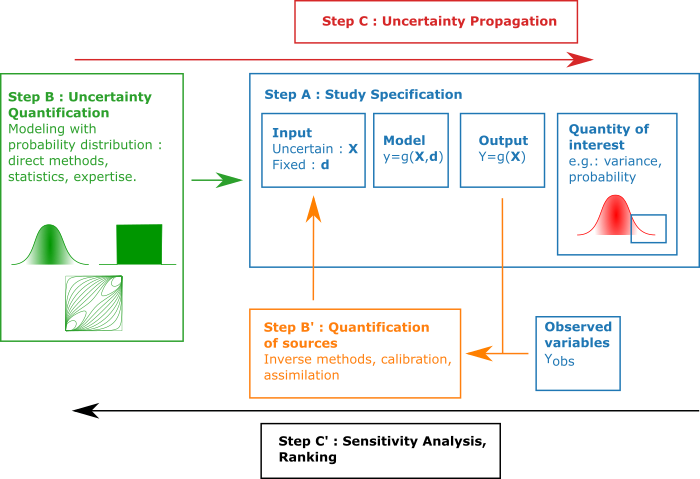
\includegraphics{MethodologieIncertitude-EN_arial.png}
\caption{ABC Methodology}
\end{figure}

\textbf{Figure 1.} Defining the physical model \(g\) is the begining of
any uncertainty study.

    \hypertarget{definition-of-a-function-in-openturns}{%
\subsection{Definition of a Function in
OpenTURNS}\label{definition-of-a-function-in-openturns}}

In OpenTURNS, a \texttt{Function} is defined from
(see \href{https://github.com/openturns/openturns/blob/18146c0a82819c3f8d8e691a119a93c155429422/lib/src/Base/Func/openturns/Function.hxx\#L74}{Function}):

\begin{itemize}
\item an evaluation which has an input \texttt{Point} and returns an output
\texttt{Point} (see
\href{https://github.com/openturns/openturns/blob/18146c0a82819c3f8d8e691a119a93c155429422/lib/src/Base/Func/openturns/Evaluation.hxx\#L83}{Evaluation})
;
\item the gradient which has an input \texttt{Point} and returns an output
\texttt{Matrix} (see
\href{https://github.com/openturns/openturns/blob/18146c0a82819c3f8d8e691a119a93c155429422/lib/src/Base/Func/openturns/GradientImplementation.hxx\#L82}{GradientImplementation})
;
\item the hessian which has an input \texttt{Point} and returns and output
\texttt{SymmetricTensor} (see
\href{https://github.com/openturns/openturns/blob/18146c0a82819c3f8d8e691a119a93c155429422/lib/src/Base/Func/openturns/HessianImplementation.hxx\#L79}{HessianImplementation}).
\end{itemize}

    \hypertarget{different-types-of-python-functions}{%
\subsection{Different types of Python
functions}\label{different-types-of-python-functions}}

\begin{longtable}[]{@{}lll@{}}
\toprule()
Type & Purpose & Implementation \\
\midrule()
\endhead
\texttt{PythonFunction} & Point to Point & \texttt{function} \\
\texttt{OpenTURNSPythonFunction} & Point to Point & \texttt{class} \\
\texttt{PythonFieldFunction} & Field to Field & \texttt{function} \\
\texttt{PythonPointToFieldFunction} & Point to Field &
\texttt{function} \\
\texttt{PythonFieldToPointFunction} & Field to Point &
\texttt{function} \\
\texttt{OpenTURNSPythonFieldFunction} & Field to Field &
\texttt{class} \\
\texttt{OpenTURNSPythonPointToFieldFunction} & Point to Field &
\texttt{class} \\
\texttt{OpenTURNSPythonFieldToPointFunction} & Field to Field &
\texttt{class} \\
\bottomrule()
\end{longtable}

\textbf{Table 1.} Different types of Python functions depending on the
inputs and outputs and the code the user must provide.

    Below is a collection of relevant and interesting help pages.

\begin{longtable}[]{@{}
  >{\raggedright\arraybackslash}p{(\columnwidth - 2\tabcolsep) * \real{0.5000}}
  >{\raggedright\arraybackslash}p{(\columnwidth - 2\tabcolsep) * \real{0.5000}}@{}}
\toprule()
\begin{minipage}[b]{\linewidth}\raggedright
Link
\end{minipage} & \begin{minipage}[b]{\linewidth}\raggedright
Type
\end{minipage} \\
\midrule()
\endhead
\href{https://openturns.github.io/openturns/latest/auto_functional_modeling/vectorial_functions/plot_quick_start_functions.html\#sphx-glr-auto-functional-modeling-vectorial-functions-plot-quick-start-functions-py}{Defining
Python and symbolic functions} & \texttt{PythonFunction} \\
\href{https://openturns.github.io/openturns/latest/auto_functional_modeling/field_functions/plot_viscous_fall_field_function.html\#sphx-glr-auto-functional-modeling-field-functions-plot-viscous-fall-field-function-py}{Define
a function with a field output} & \texttt{PythonPointToFieldFunction} \\
\href{https://openturns.github.io/openturns/latest/developer_guide/wrapper_development.html}{Wrapper
development} & \texttt{coupling\_tools} \\
\bottomrule()
\end{longtable}

\textbf{Table 2.} Help pages which present the use of Python functions.

    \hypertarget{why-may-we-use-a-python-function}{%
\subsection{Why may we use a Python
function?}\label{why-may-we-use-a-python-function}}

There are several reasons to use a Python function.

\begin{itemize}
\tightlist
\item
  Use \textbf{existing Python code} implementing a physical model \(g\).
  This model may use \texttt{numpy}, \texttt{scipy} or a dedicated API
  (e.g.~\texttt{AsterStudy} or \texttt{Telemac}).
\item
  Achieve a \textbf{great flexibility} in the code, involving several
  other Python functions or classes.
\item
  Provide the code to \textbf{another user}, with the possibility to
  \textbf{maintain the code} easily.
\item
  Get \textbf{performance} by parallelizing the evaluation.
\end{itemize}

    \hypertarget{what-is-the-pythonfunction-necessary-and-useful}{%
\subsection{What is the PythonFunction necessary and
useful?}\label{what-is-the-pythonfunction-necessary-and-useful}}

Surprise for a Python user:

\begin{itemize}
\tightlist
\item
  Providing a \texttt{PythonFunction} class in a Python library may seem
  surprising.
\item
  Other libraries (e.g.~\texttt{scipy}) do not require that.
\end{itemize}

Discussion:

\begin{itemize}
\tightlist
\item
  The \texttt{PythonFunction} is \textbf{necessary}, because OpenTURNS
  is a C++ library accessible through SWIG.
\item
  It is \textbf{useful}, because OpenTURNS provides many different types
  of functions so that each algorithm can be as efficient as possible.
\end{itemize}

Examples:

\begin{itemize}
\tightlist
\item
  The \texttt{ParametricFunction} class is useful for calibration
  algorithms.
\item
  The \texttt{DistanceToDomainFunction} class is useful for HSIC
  indices.
\item
  The \texttt{Point(or\ Field)toPoint(or\ Field)Function} is class is
  useful for stochastic processes.
\end{itemize}

    \hypertarget{the-simplest-possible-example}{%
\subsection{The simplest possible
example}\label{the-simplest-possible-example}}

    \begin{tcolorbox}[breakable, size=fbox, boxrule=1pt, pad at break*=1mm,colback=cellbackground, colframe=cellborder]
\prompt{In}{incolor}{2}{\boxspacing}
\begin{Verbatim}[commandchars=\\\{\}]
\PY{k}{def} \PY{n+nf}{mySimulator}\PY{p}{(}\PY{n}{x}\PY{p}{)}\PY{p}{:}
    \PY{n}{y0} \PY{o}{=} \PY{n}{x}\PY{p}{[}\PY{l+m+mi}{0}\PY{p}{]} \PY{o}{+} \PY{n}{x}\PY{p}{[}\PY{l+m+mi}{1}\PY{p}{]} \PY{o}{+} \PY{n}{x}\PY{p}{[}\PY{l+m+mi}{2}\PY{p}{]}
    \PY{n}{y1} \PY{o}{=} \PY{n}{x}\PY{p}{[}\PY{l+m+mi}{0}\PY{p}{]} \PY{o}{\PYZhy{}} \PY{n}{x}\PY{p}{[}\PY{l+m+mi}{1}\PY{p}{]} \PY{o}{*} \PY{n}{x}\PY{p}{[}\PY{l+m+mi}{2}\PY{p}{]}
    \PY{n}{y} \PY{o}{=} \PY{p}{[}\PY{n}{y0}\PY{p}{,} \PY{n}{y1}\PY{p}{]}  \PY{c+c1}{\PYZsh{} Will be converted to a Point by SWIG}
    \PY{k}{return} \PY{n}{y}


\PY{n}{gFunction} \PY{o}{=} \PY{n}{ot}\PY{o}{.}\PY{n}{PythonFunction}\PY{p}{(}\PY{l+m+mi}{3}\PY{p}{,} \PY{l+m+mi}{2}\PY{p}{,} \PY{n}{mySimulator}\PY{p}{)}
\PY{n}{x} \PY{o}{=} \PY{p}{[}\PY{l+m+mf}{1.0}\PY{p}{]} \PY{o}{*} \PY{l+m+mi}{3}  \PY{c+c1}{\PYZsh{} Will be converted to a Point by SWIG}
\PY{n+nb}{print}\PY{p}{(}\PY{l+s+s2}{\PYZdq{}}\PY{l+s+s2}{x = }\PY{l+s+s2}{\PYZdq{}}\PY{p}{,} \PY{n}{x}\PY{p}{)}
\PY{n}{y} \PY{o}{=} \PY{n}{gFunction}\PY{p}{(}\PY{n}{x}\PY{p}{)}
\PY{n+nb}{print}\PY{p}{(}\PY{l+s+s2}{\PYZdq{}}\PY{l+s+s2}{y = }\PY{l+s+s2}{\PYZdq{}}\PY{p}{,} \PY{n}{y}\PY{p}{)}
\end{Verbatim}
\end{tcolorbox}

    \begin{Verbatim}[commandchars=\\\{\}]
x =  [1.0, 1.0, 1.0]
y =  [3,0]
    \end{Verbatim}

    \hypertarget{other-ways-to-implement-a-function}{%
\subsection{Other ways to implement a
function}\label{other-ways-to-implement-a-function}}

We may also consider other ways to implement a function.

\begin{longtable}[]{@{}
  >{\raggedright\arraybackslash}p{(\columnwidth - 4\tabcolsep) * \real{0.3333}}
  >{\raggedright\arraybackslash}p{(\columnwidth - 4\tabcolsep) * \real{0.3333}}
  >{\raggedright\arraybackslash}p{(\columnwidth - 4\tabcolsep) * \real{0.3333}}@{}}
\toprule()
\begin{minipage}[b]{\linewidth}\raggedright
Class
\end{minipage} & \begin{minipage}[b]{\linewidth}\raggedright
Advantages
\end{minipage} & \begin{minipage}[b]{\linewidth}\raggedright
Drawbacks
\end{minipage} \\
\midrule()
\endhead
\texttt{PythonFunction} & Flexible & Not always the fastest \\
\texttt{SymbolicFunction} & Exact gradient (not always), fast (not
always) & Limited features \\
\bottomrule()
\end{longtable}

\textbf{Table 3.} Comparison of Python and symbolic functions.

    \begin{longtable}[]{@{}
  >{\raggedright\arraybackslash}p{(\columnwidth - 6\tabcolsep) * \real{0.2500}}
  >{\raggedright\arraybackslash}p{(\columnwidth - 6\tabcolsep) * \real{0.2500}}
  >{\raggedright\arraybackslash}p{(\columnwidth - 6\tabcolsep) * \real{0.2500}}
  >{\raggedright\arraybackslash}p{(\columnwidth - 6\tabcolsep) * \real{0.2500}}@{}}
\toprule()
\begin{minipage}[b]{\linewidth}\raggedright
Tool
\end{minipage} & \begin{minipage}[b]{\linewidth}\raggedright
Features
\end{minipage} & \begin{minipage}[b]{\linewidth}\raggedright
Pros/Cons
\end{minipage} & \begin{minipage}[b]{\linewidth}\raggedright
Link
\end{minipage} \\
\midrule()
\endhead
Otwrapy & Multithread, distributed evaluation & Can be fast, depending
on the situation &
\href{https://openturns.github.io/otwrapy/master/}{doc} \\
Autograd & Automatic differentiation & Not always possible &
\href{https://github.com/HIPS/autograd}{doc} \\
Jax & Automatic differentiation & Not always possible &
\href{https://github.com/google/jax}{doc} \\
\texttt{coupling\_tools} & Connect to an external program using files &
Slow (depends on the speed of the disk) &
\href{https://openturns.github.io/openturns/latest/developer_guide/wrapper_development.html}{doc} \\
\bottomrule()
\end{longtable}

\textbf{Table 4.} Tools to consider when using a Python function.

More details : - See \texttt{Coupling\ Tools.ipynb} in this repository
for details on \texttt{coupling\_tools}. - More details on
\texttt{Otwrapy} and \texttt{Jax} latex in the slides.

    \hypertarget{benchmark}{%
\subsection{Benchmark}\label{benchmark}}

We consider the function \(g : \mathbb{R}^3 \rightarrow \mathbb{R}^2\):
\[
\begin{aligned}
    y_0 &= x_1 + x_2 + x_3 \\
    y_1 &= x_1 - x_2 x_3
\end{aligned}
\] for any \(\boldsymbol{x}\in \mathbb{R}^3\).

\begin{itemize}
\tightlist
\item
  The input distribution has \(\mathcal{N}(0,1)\) independent marginals
  : generating the input sample is fast.
\item
  We call the \texttt{getSample()} method of the output random vector.
\item
  The evaluation is relatively fast.
\item
  The vectorization is achieved using the \texttt{func\_sample} keyword
  and the \texttt{numpy} library.
\end{itemize}

    \begin{figure}
\centering
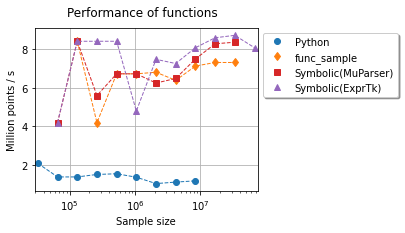
\includegraphics{wrapper-python-benchmark.png}
\caption{Python benchmark}
\end{figure}

\textbf{Figure 2.} A benchmark of two Python functions compared to a symbolic
function (see \texttt{python\_benchmark.py}).

We see that, on this example, the two fastest methods are the symbol
function and the vectorised Python functions.

    Comments :

\begin{itemize}
\item
  See also the benchmark available
  \href{https://openturns.github.io/openturns/latest/developer_guide/wrapper_development.html\#performance-considerations}{in
  the doc}.
\item
  The performance of the symbolic function may depend on the backend
  \texttt{ExprTk} or \texttt{MuParser}. This can be configured using the
  \texttt{SymbolicParser-Backend} key of the \texttt{ResourceMap}.
\end{itemize}

    \begin{tcolorbox}[breakable, size=fbox, boxrule=1pt, pad at break*=1mm,colback=cellbackground, colframe=cellborder]
\prompt{In}{incolor}{3}{\boxspacing}
\begin{Verbatim}[commandchars=\\\{\}]
\PY{n}{ot}\PY{o}{.}\PY{n}{ResourceMap}\PY{o}{.}\PY{n}{Set}\PY{p}{(}\PY{l+s+s2}{\PYZdq{}}\PY{l+s+s2}{SymbolicParser\PYZhy{}Backend}\PY{l+s+s2}{\PYZdq{}}\PY{p}{,} \PY{l+s+s2}{\PYZdq{}}\PY{l+s+s2}{ExprTk}\PY{l+s+s2}{\PYZdq{}}\PY{p}{)}  \PY{c+c1}{\PYZsh{} The default}
\PY{n}{ot}\PY{o}{.}\PY{n}{ResourceMap}\PY{o}{.}\PY{n}{Set}\PY{p}{(}\PY{l+s+s2}{\PYZdq{}}\PY{l+s+s2}{SymbolicParser\PYZhy{}Backend}\PY{l+s+s2}{\PYZdq{}}\PY{p}{,} \PY{l+s+s2}{\PYZdq{}}\PY{l+s+s2}{MuParser}\PY{l+s+s2}{\PYZdq{}}\PY{p}{)}
\end{Verbatim}
\end{tcolorbox}

    \hypertarget{how-can-pythonfunction-be-made-fast}{%
\subsection{How can PythonFunction be made
fast?}\label{how-can-pythonfunction-be-made-fast}}

The \texttt{PythonFunction} is based on the
\texttt{OpenTURNSPythonFunction} than we will present later in the
slides.

Depending on the \texttt{func\_sample} and \texttt{n\_cpus} options, we
can make the evaluation faster. 
\begin{itemize}
\item \texttt{func\_sample}: evaluate the
function on a \texttt{Sample} instead of a \texttt{Point} to vectorize
the evaluations~;

\item \texttt{n\_cpus}: uses \texttt{multiprocessing} to
make the evaluations parallel.
\end{itemize}

    Here are different cases, depending the options specified by the user:
    \begin{itemize}
\item If \texttt{func\_sample} is undefined and \texttt{n\_cpus} is undefined
(i.e.~the default), then the user-provided \texttt{func} function is
used. It is not made parallel by OpenTURNS (but the user can do so).

\item If \texttt{func\_sample} is undefined and \texttt{n\_cpus} is defined,
then the implementa\-tion uses \texttt{mul\-ti\-processing}'s \texttt{Pool} to
make the evaluation parallel (see the details in the private method
\href{https://github.com/openturns/openturns/blob/18146c0a82819c3f8d8e691a119a93c155429422/python/src/Function.i\#L213}{\texttt{\_exec\_sample\_multiprocessing\_func}}).

\item If \texttt{func\_sample} and \texttt{n\_cpus} are both defined, then
the implementation uses divides the \texttt{Sample} into sub-samples
which are evaluated in parallel (see the details in the private method 
\href{https://github.com/openturns/openturns/blob/18146c0a82819c3f8d8e691a119a93c155429422/python/src/Function.i\#L282}{\texttt{\_exec\_sample\_multiprocessing\_func\_sample}}).
\end{itemize}

    \hypertarget{what-is-the-memoryview-class}{%
\subsection{What is the memoryview
class?}\label{what-is-the-memoryview-class}}

The \texttt{memoryview} object is the type of object we receive as input
to a \texttt{PythonFunction}.

This class provides a lightweight object which prevent unnecessary
object copies which can make the evaluation slower.

    \begin{tcolorbox}[breakable, size=fbox, boxrule=1pt, pad at break*=1mm,colback=cellbackground, colframe=cellborder]
\prompt{In}{incolor}{4}{\boxspacing}
\begin{Verbatim}[commandchars=\\\{\}]
\PY{k}{def} \PY{n+nf}{mySimulator}\PY{p}{(}\PY{n}{x}\PY{p}{)}\PY{p}{:}
    \PY{n+nb}{print}\PY{p}{(}\PY{l+s+s2}{\PYZdq{}}\PY{l+s+s2}{Type of x : }\PY{l+s+s2}{\PYZdq{}}\PY{p}{,} \PY{n+nb}{type}\PY{p}{(}\PY{n}{x}\PY{p}{)}\PY{p}{)}
    \PY{c+c1}{\PYZsh{} dimension = x.getDimension()  \PYZsh{} Fail}
    \PY{n}{y0} \PY{o}{=} \PY{n}{x}\PY{p}{[}\PY{l+m+mi}{0}\PY{p}{]} \PY{o}{+} \PY{n}{x}\PY{p}{[}\PY{l+m+mi}{1}\PY{p}{]} \PY{o}{+} \PY{n}{x}\PY{p}{[}\PY{l+m+mi}{2}\PY{p}{]}
    \PY{n}{y1} \PY{o}{=} \PY{n}{x}\PY{p}{[}\PY{l+m+mi}{0}\PY{p}{]} \PY{o}{\PYZhy{}} \PY{n}{x}\PY{p}{[}\PY{l+m+mi}{1}\PY{p}{]} \PY{o}{*} \PY{n}{x}\PY{p}{[}\PY{l+m+mi}{2}\PY{p}{]}
    \PY{n}{y} \PY{o}{=} \PY{p}{[}\PY{n}{y0}\PY{p}{,} \PY{n}{y1}\PY{p}{]}
    \PY{k}{return} \PY{n}{y}


\PY{n}{gFunction} \PY{o}{=} \PY{n}{ot}\PY{o}{.}\PY{n}{PythonFunction}\PY{p}{(}\PY{l+m+mi}{3}\PY{p}{,} \PY{l+m+mi}{2}\PY{p}{,} \PY{n}{mySimulator}\PY{p}{)}
\PY{n}{x} \PY{o}{=} \PY{p}{[}\PY{l+m+mf}{1.0}\PY{p}{]} \PY{o}{*} \PY{l+m+mi}{3}
\PY{n+nb}{print}\PY{p}{(}\PY{l+s+s2}{\PYZdq{}}\PY{l+s+s2}{x = }\PY{l+s+s2}{\PYZdq{}}\PY{p}{,} \PY{n}{x}\PY{p}{)}
\PY{n}{y} \PY{o}{=} \PY{n}{gFunction}\PY{p}{(}\PY{n}{x}\PY{p}{)}
\PY{n+nb}{print}\PY{p}{(}\PY{l+s+s2}{\PYZdq{}}\PY{l+s+s2}{y = }\PY{l+s+s2}{\PYZdq{}}\PY{p}{,} \PY{n}{y}\PY{p}{)}
\end{Verbatim}
\end{tcolorbox}

    \begin{Verbatim}[commandchars=\\\{\}]
x =  [1.0, 1.0, 1.0]
Type of x :  <class 'openturns.memoryview.Buffer'>
y =  [3,0]
    \end{Verbatim}

    The method \texttt{x.getDimension()} fails:

\begin{verbatim}
AttributeError: 'openturns.memoryview.Buffer' 
  object has no attribute 'getDimension'
\end{verbatim}

From the
\href{https://openturns.github.io/openturns/latest/user_manual/_generated/openturns.PythonFunction.html\#}{doc}:

\emph{``For efficiency reasons, these functions do not receive a
\texttt{Point} or \texttt{Sample} as arguments, but a proxy object which
gives access to internal object data. This object supports indexing, but
nothing more. It must be wrapped into another object, for instance
\texttt{Point} in \texttt{func} and \texttt{Sample} in
\texttt{func\_sample}, or in a Numpy \texttt{array}, for vectorized
operations.''}

    If we have to , we can convert the \texttt{memoryview} into a
\texttt{Point}: this can make the evaluation slower, but can be
necessary in some situations.

    \begin{tcolorbox}[breakable, size=fbox, boxrule=1pt, pad at break*=1mm,colback=cellbackground, colframe=cellborder]
\prompt{In}{incolor}{5}{\boxspacing}
\begin{Verbatim}[commandchars=\\\{\}]
\PY{k}{def} \PY{n+nf}{mySimulator}\PY{p}{(}\PY{n}{x}\PY{p}{)}\PY{p}{:}
    \PY{n}{x} \PY{o}{=} \PY{n}{ot}\PY{o}{.}\PY{n}{Point}\PY{p}{(}\PY{n}{x}\PY{p}{)}  \PY{c+c1}{\PYZsh{} Convert to Point, but only if necessary}
    \PY{n+nb}{print}\PY{p}{(}\PY{l+s+s2}{\PYZdq{}}\PY{l+s+s2}{Type of x : }\PY{l+s+s2}{\PYZdq{}}\PY{p}{,} \PY{n+nb}{type}\PY{p}{(}\PY{n}{x}\PY{p}{)}\PY{p}{)}
    \PY{n}{dimension} \PY{o}{=} \PY{n}{x}\PY{o}{.}\PY{n}{getDimension}\PY{p}{(}\PY{p}{)}  \PY{c+c1}{\PYZsh{} Ok}
    \PY{n}{y0} \PY{o}{=} \PY{l+m+mf}{0.0}
    \PY{k}{for} \PY{n}{i} \PY{o+ow}{in} \PY{n+nb}{range}\PY{p}{(}\PY{n}{dimension}\PY{p}{)}\PY{p}{:}
        \PY{n}{y0} \PY{o}{+}\PY{o}{=} \PY{n}{x}\PY{p}{[}\PY{n}{i}\PY{p}{]}
    \PY{n}{y1} \PY{o}{=} \PY{n}{x}\PY{p}{[}\PY{l+m+mi}{0}\PY{p}{]} \PY{o}{\PYZhy{}} \PY{n}{x}\PY{p}{[}\PY{l+m+mi}{1}\PY{p}{]} \PY{o}{*} \PY{n}{x}\PY{p}{[}\PY{l+m+mi}{2}\PY{p}{]}
    \PY{n}{y} \PY{o}{=} \PY{p}{[}\PY{n}{y0}\PY{p}{,} \PY{n}{y1}\PY{p}{]}
    \PY{k}{return} \PY{n}{y}


\PY{n}{gFunction} \PY{o}{=} \PY{n}{ot}\PY{o}{.}\PY{n}{PythonFunction}\PY{p}{(}\PY{l+m+mi}{3}\PY{p}{,} \PY{l+m+mi}{2}\PY{p}{,} \PY{n}{mySimulator}\PY{p}{)}
\PY{n}{x} \PY{o}{=} \PY{p}{[}\PY{l+m+mf}{1.0}\PY{p}{]} \PY{o}{*} \PY{l+m+mi}{3}
\PY{n}{gFunction}\PY{p}{(}\PY{n}{x}\PY{p}{)}
\end{Verbatim}
\end{tcolorbox}

    \begin{Verbatim}[commandchars=\\\{\}]
Type of x :  <class 'openturns.typ.Point'>
    \end{Verbatim}

            \begin{tcolorbox}[breakable, size=fbox, boxrule=.5pt, pad at break*=1mm, opacityfill=0]
\prompt{Out}{outcolor}{5}{\boxspacing}
\begin{Verbatim}[commandchars=\\\{\}]
class=Point name=Unnamed dimension=2 values=[3,0]
\end{Verbatim}
\end{tcolorbox}
        
    \hypertarget{what-is-the-parametricfunction-for}{%
\subsection{What is the ParametricFunction
for?}\label{what-is-the-parametricfunction-for}}

There are some cases when we want to create a function which has
parameters, e.g. the gravity of Earth $g = 9.81$ $m/s^2$.
The \texttt{ParametricFunction} can be considered when the
parameters is a vector of points:

\begin{itemize}
\tightlist
\item
  to perform
  \href{https://openturns.github.io/openturns/latest/auto_calibration/least_squares_and_gaussian_calibration/plot_calibration_deflection_tube.html\#sphx-glr-auto-calibration-least-squares-and-gaussian-calibration-plot-calibration-deflection-tube-py}{Calibration
  using least squares} : the parameter to calibrate is the parameter of
  the \texttt{ParametricFunction} ;
\item
  to perform
  \href{https://openturns.github.io/openturns/latest/auto_calibration/bayesian_calibration/plot_bayesian_calibration_flooding.html}{Bayesian
  calibration} : the input of the \texttt{ParametricFunction} function
  is the parameter for which we want the \emph{posterior} distribution ;
\item
  to solve optimization problems with a parametric function (which
  avoids to create a new function each time the parameters change) ;
\item
  etc.
\end{itemize}

We consider here the Ishigami test function.

\hypertarget{references}{%
\subsubsection{References}\label{references}}

\begin{itemize}
\tightlist
\item
  Ishigami, T., Homma, T. (1990, December). An importance quantification
  technique in uncertainty analysis for computer models. In Uncertainty
  Modeling and Analysis, 1990. Proceedings., First International
  Symposium on (pp.~398-403). IEEE.
\end{itemize}

    \begin{tcolorbox}[breakable, size=fbox, boxrule=1pt, pad at break*=1mm,colback=cellbackground, colframe=cellborder]
\prompt{In}{incolor}{6}{\boxspacing}
\begin{Verbatim}[commandchars=\\\{\}]
\PY{k}{def} \PY{n+nf}{ishigami}\PY{p}{(}\PY{n}{x}\PY{p}{)}\PY{p}{:}
    \PY{n}{x0}\PY{p}{,} \PY{n}{x1}\PY{p}{,} \PY{n}{x2}\PY{p}{,} \PY{n}{a}\PY{p}{,} \PY{n}{b} \PY{o}{=} \PY{n}{x}
    \PY{n}{y0} \PY{o}{=} \PY{n}{np}\PY{o}{.}\PY{n}{sin}\PY{p}{(}\PY{n}{x0}\PY{p}{)} \PY{o}{+} \PY{n}{a} \PY{o}{*} \PY{n}{np}\PY{o}{.}\PY{n}{sin}\PY{p}{(}\PY{n}{x1}\PY{p}{)} \PY{o}{*}\PY{o}{*} \PY{l+m+mi}{2} \PY{o}{+} \PY{n}{b} \PY{o}{*} \PY{n}{x2}\PY{o}{*}\PY{o}{*}\PY{l+m+mi}{4} \PY{o}{*} \PY{n}{np}\PY{o}{.}\PY{n}{sin}\PY{p}{(}\PY{n}{x0}\PY{p}{)}
    \PY{n}{y} \PY{o}{=} \PY{p}{[}\PY{n}{y0}\PY{p}{]}
    \PY{k}{return} \PY{n}{y}


\PY{n}{gFunctionFull} \PY{o}{=} \PY{n}{ot}\PY{o}{.}\PY{n}{PythonFunction}\PY{p}{(}\PY{l+m+mi}{5}\PY{p}{,} \PY{l+m+mi}{1}\PY{p}{,} \PY{n}{ishigami}\PY{p}{)}
\PY{n}{a} \PY{o}{=} \PY{l+m+mf}{7.0}
\PY{n}{b} \PY{o}{=} \PY{l+m+mf}{0.1}
\PY{n}{xFull} \PY{o}{=} \PY{p}{[}\PY{l+m+mf}{0.5}\PY{p}{,} \PY{l+m+mf}{1.0}\PY{p}{,} \PY{l+m+mf}{1.5}\PY{p}{,} \PY{n}{a}\PY{p}{,} \PY{n}{b}\PY{p}{]}
\PY{n}{y} \PY{o}{=} \PY{n}{gFunctionFull}\PY{p}{(}\PY{n}{xFull}\PY{p}{)}
\PY{n+nb}{print}\PY{p}{(}\PY{n}{y}\PY{p}{)}
\end{Verbatim}
\end{tcolorbox}

    \begin{Verbatim}[commandchars=\\\{\}]
[5.67865]
    \end{Verbatim}

    To propage the uncertainty through the Ishigami function, we can set the
parameters \(a\) and \(b\), so that the function only has
\texttt{(x1,\ x2,\ x3)} as input.

Please use the
\href{https://openturns.github.io/openturns/latest/usecases/use_case_ishigami.html}{Ishigami}
from the library for real simulations.

    The next table presents the mapping from the variable name to its index.
Notice that Python have indices that start from 0. The
\texttt{gFunctionFull} function has no parameters.

\begin{longtable}[]{@{}ll@{}}
\toprule()
Input variable & Input index \\
\midrule()
\endhead
\(x_1\) & 0 \\
\(x_2\) & 1 \\
\(x_3\) & 2 \\
\(a\) & 3 \\
\(b\) & 4 \\
\bottomrule()
\end{longtable}

\begin{longtable}[]{@{}ll@{}}
\toprule()
Parameter & Parameter index \\
\midrule()
\endhead
$\emptyset$ & $\emptyset$ \\
\bottomrule()
\end{longtable}

\textbf{Table 5.} Input variables and parameters of the (full)
\texttt{gFunctionFull} function.

    \begin{tcolorbox}[breakable, size=fbox, boxrule=1pt, pad at break*=1mm,colback=cellbackground, colframe=cellborder]
\prompt{In}{incolor}{7}{\boxspacing}
\begin{Verbatim}[commandchars=\\\{\}]
\PY{n}{indices} \PY{o}{=} \PY{p}{[}\PY{l+m+mi}{3}\PY{p}{,} \PY{l+m+mi}{4}\PY{p}{]}
\PY{n}{referencePoint} \PY{o}{=} \PY{p}{[}\PY{n}{a}\PY{p}{,} \PY{n}{b}\PY{p}{]}
\PY{n}{gFunction} \PY{o}{=} \PY{n}{ot}\PY{o}{.}\PY{n}{ParametricFunction}\PY{p}{(}\PY{n}{gFunctionFull}\PY{p}{,} \PY{n}{indices}\PY{p}{,} \PY{n}{referencePoint}\PY{p}{)}
\PY{n}{x} \PY{o}{=} \PY{p}{[}\PY{l+m+mf}{0.5}\PY{p}{,} \PY{l+m+mf}{1.0}\PY{p}{,} \PY{l+m+mf}{1.5}\PY{p}{]}
\PY{n}{y} \PY{o}{=} \PY{n}{gFunction}\PY{p}{(}\PY{n}{x}\PY{p}{)}
\PY{n+nb}{print}\PY{p}{(}\PY{n}{y}\PY{p}{)}
\end{Verbatim}
\end{tcolorbox}

    \begin{Verbatim}[commandchars=\\\{\}]
[5.67865]
    \end{Verbatim}

    Manage parameters:

\begin{itemize}
\tightlist
\item
  We can use the \texttt{setParameter()} to set the parameters (and
  \texttt{getParameter()} to get them).
\item
  The \texttt{parameterGradient()} returns the gradient of the function
  with respect to the parameters.
\end{itemize}

    \begin{tcolorbox}[breakable, size=fbox, boxrule=1pt, pad at break*=1mm,colback=cellbackground, colframe=cellborder]
\prompt{In}{incolor}{8}{\boxspacing}
\begin{Verbatim}[commandchars=\\\{\}]
\PY{n+nb}{print}\PY{p}{(}\PY{n}{gFunction}\PY{o}{.}\PY{n}{getParameter}\PY{p}{(}\PY{p}{)}\PY{p}{)}
\PY{n}{gFunction}\PY{o}{.}\PY{n}{setParameter}\PY{p}{(}\PY{p}{[}\PY{l+m+mf}{8.0}\PY{p}{,} \PY{l+m+mf}{0.2}\PY{p}{]}\PY{p}{)}
\PY{n+nb}{print}\PY{p}{(}\PY{n}{gFunction}\PY{o}{.}\PY{n}{getParameter}\PY{p}{(}\PY{p}{)}\PY{p}{)}
\end{Verbatim}
\end{tcolorbox}

    \begin{Verbatim}[commandchars=\\\{\}]
[7,0.1]
[8,0.2]
    \end{Verbatim}

    The next table present the inputs and parameters of the parametric
\texttt{gFunction} function. It has 3 inputs and 2 parameters.

\begin{longtable}[]{@{}ll@{}}
\toprule()
Input variable & Input index \\
\midrule()
\endhead
\(x_1\) & 0 \\
\(x_2\) & 1 \\
\(x_3\) & 2 \\
\bottomrule()
\end{longtable}

\begin{longtable}[]{@{}ll@{}}
\toprule()
Parameter & Parameter index \\
\midrule()
\endhead
\(a\) & 0 \\
\(b\) & 1 \\
\bottomrule()
\end{longtable}

\textbf{Table 6.} Input variables and parameters of the (parametric)
\texttt{gFunction} function.

    \hypertarget{why-is-the-openturnspythonfunction-class-most-powerful}{%
\subsection{Why is the OpenTURNSPythonFunction class most
powerful?}\label{why-is-the-openturnspythonfunction-class-most-powerful}}

When the parameters cannot be stored as a single \texttt{Point}, we need
a more powerful tool: the \texttt{OpenTURNSPythonFunction} class
provides a way to implement a class so that we can provide any necessary
parameter (whatever its type) to the evaluation.
\begin{itemize}
\item The constructor of
the object can have any number or type of input arguments, as any
\texttt{Class} object in Python.
\item The calculations which are done in
the constructor are done \emph{``once for all''} at the creation of the
object, which can make some calculations faster.
\end{itemize}

    \begin{tcolorbox}[breakable, size=fbox, boxrule=1pt, pad at break*=1mm,colback=cellbackground, colframe=cellborder]
\prompt{In}{incolor}{9}{\boxspacing}
\begin{Verbatim}[commandchars=\\\{\}]
\PY{k}{class} \PY{n+nc}{IshigamiFunction}\PY{p}{(}\PY{n}{ot}\PY{o}{.}\PY{n}{OpenTURNSPythonFunction}\PY{p}{)}\PY{p}{:}
    \PY{k}{def} \PY{n+nf+fm}{\PYZus{}\PYZus{}init\PYZus{}\PYZus{}}\PY{p}{(}\PY{n+nb+bp}{self}\PY{p}{,} \PY{n}{a}\PY{p}{,} \PY{n}{b}\PY{p}{)}\PY{p}{:}
        \PY{n+nb}{super}\PY{p}{(}\PY{p}{)}\PY{o}{.}\PY{n+nf+fm}{\PYZus{}\PYZus{}init\PYZus{}\PYZus{}}\PY{p}{(}\PY{l+m+mi}{3}\PY{p}{,} \PY{l+m+mi}{1}\PY{p}{)}
        \PY{n+nb+bp}{self}\PY{o}{.}\PY{n}{a} \PY{o}{=} \PY{n}{a}
        \PY{n+nb+bp}{self}\PY{o}{.}\PY{n}{b} \PY{o}{=} \PY{n}{b}

    \PY{k}{def} \PY{n+nf}{\PYZus{}exec}\PY{p}{(}\PY{n+nb+bp}{self}\PY{p}{,} \PY{n}{x}\PY{p}{)}\PY{p}{:}
        \PY{n}{y0} \PY{o}{=} \PY{p}{(}
            \PY{n}{np}\PY{o}{.}\PY{n}{sin}\PY{p}{(}\PY{n}{x}\PY{p}{[}\PY{l+m+mi}{0}\PY{p}{]}\PY{p}{)}
            \PY{o}{+} \PY{n+nb+bp}{self}\PY{o}{.}\PY{n}{a} \PY{o}{*} \PY{n}{np}\PY{o}{.}\PY{n}{sin}\PY{p}{(}\PY{n}{x}\PY{p}{[}\PY{l+m+mi}{1}\PY{p}{]}\PY{p}{)} \PY{o}{*}\PY{o}{*} \PY{l+m+mi}{2}
            \PY{o}{+} \PY{n+nb+bp}{self}\PY{o}{.}\PY{n}{b} \PY{o}{*} \PY{n}{x}\PY{p}{[}\PY{l+m+mi}{2}\PY{p}{]} \PY{o}{*}\PY{o}{*} \PY{l+m+mi}{4} \PY{o}{*} \PY{n}{np}\PY{o}{.}\PY{n}{sin}\PY{p}{(}\PY{n}{x}\PY{p}{[}\PY{l+m+mi}{0}\PY{p}{]}\PY{p}{)}
        \PY{p}{)}
        \PY{k}{return} \PY{p}{[}\PY{n}{y0}\PY{p}{]}
\end{Verbatim}
\end{tcolorbox}

    \begin{tcolorbox}[breakable, size=fbox, boxrule=1pt, pad at break*=1mm,colback=cellbackground, colframe=cellborder]
\prompt{In}{incolor}{10}{\boxspacing}
\begin{Verbatim}[commandchars=\\\{\}]
\PY{n}{a} \PY{o}{=} \PY{l+m+mf}{7.0}
\PY{n}{b} \PY{o}{=} \PY{l+m+mf}{0.1}
\PY{n}{ishigamiFunction} \PY{o}{=} \PY{n}{IshigamiFunction}\PY{p}{(}\PY{n}{a}\PY{p}{,} \PY{n}{b}\PY{p}{)}  \PY{c+c1}{\PYZsh{} Create the object}
\PY{n}{gFunction} \PY{o}{=} \PY{n}{ot}\PY{o}{.}\PY{n}{Function}\PY{p}{(}\PY{n}{ishigamiFunction}\PY{p}{)}  \PY{c+c1}{\PYZsh{} Convert to a Function}
\PY{n}{x} \PY{o}{=} \PY{p}{[}\PY{l+m+mf}{0.5}\PY{p}{,} \PY{l+m+mf}{1.0}\PY{p}{,} \PY{l+m+mf}{1.5}\PY{p}{]}
\PY{n}{y} \PY{o}{=} \PY{n}{gFunction}\PY{p}{(}\PY{n}{x}\PY{p}{)}
\PY{n+nb}{print}\PY{p}{(}\PY{n}{y}\PY{p}{)}
\end{Verbatim}
\end{tcolorbox}

    \begin{Verbatim}[commandchars=\\\{\}]
[5.67865]
    \end{Verbatim}

    Other examples:
\begin{itemize}
\item in the PRACE training
\href{https://github.com/mbaudin47/hpcuqtraining/blob/773ddaed56339ddb548f82a2ff16bfcf5c00be2c/2019/Scripts/wrapper.py}{a
wrapper to the cantilever beam} ;
\item in otbenchmark, the
\href{https://github.com/mbaudin47/otbenchmark/blob/f33a9c6694cc0bb3e2680164519b82e9f2983977/otbenchmark/DirichletSensitivity.py}{Dirichlet}
test function for sensitivity analysis ;
\item in otbenchmark, the
\href{https://github.com/mbaudin47/otbenchmark/blob/f33a9c6694cc0bb3e2680164519b82e9f2983977/examples/scripts/testCrue-classeOTPFun.py}{flooding}
test case ;
\item in otbenchmark, the
\href{https://github.com/mbaudin47/otbenchmark/blob/f33a9c6694cc0bb3e2680164519b82e9f2983977/otbenchmark/MorrisSensitivity.py}{Morris}
test function.
\end{itemize}

    \hypertarget{otwrapy}{%
\subsection{Otwrapy}\label{otwrapy}}

The \texttt{otwrapy} package (available at
\href{https://github.com/openturns/otwrapy}{github}) provides a
\texttt{Parallelizer} class that converts any \texttt{ot.Function} into
a parallel wrapper using either \texttt{multiprocessing},
\texttt{ipyparallel}, \texttt{joblib} or \texttt{pathos}.

See the
\href{https://felipeam86.github.io/HPC-Uncertainties-PRACE/}{slides}
from Felipe Aguirre Martinez for Otwrapy details.

To install \texttt{otwrapy}, use conda
(\href{https://anaconda.org/conda-forge/otwrapy}{package}):

\begin{Shaded}
\begin{Highlighting}[]
\ExtensionTok{$}\NormalTok{ conda install }\AttributeTok{{-}c}\NormalTok{ conda{-}forge otwrapy}
\end{Highlighting}
\end{Shaded}

The \texttt{Parallelizer} class parallelize a \texttt{Function}:

\begin{Shaded}
\begin{Highlighting}[]
\ImportTok{import}\NormalTok{ otwrapy }\ImportTok{as}\NormalTok{ otw}
\ImportTok{from}\NormalTok{ otwrapy.examples.beam }\ImportTok{import}\NormalTok{ Wrapper}
\NormalTok{parallelized\_beam\_wrapper }\OperatorTok{=}\NormalTok{ otw.Parallelizer(Wrapper())}
\end{Highlighting}
\end{Shaded}

    \begin{figure}
\centering
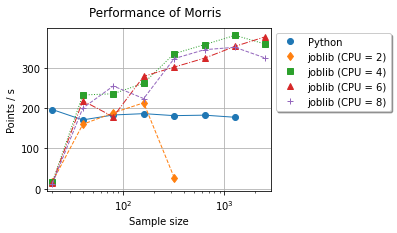
\includegraphics{benchmark_Morris_otwrapy.png}
\caption{Python benchmark}
\end{figure}

\textbf{Figure 2.} A benchmark of Morris function from \texttt{otmorris}
using \texttt{otwrapy} (see the implementation details in \texttt{benchmark\_Morris\_otwrapy.py}).

We see that, on this example, the ``joblib'' backend improves the
performance when the number of CPUs is in the range \([4, 6]\). Using
more CPUs decreases the performance.

    \hypertarget{jax}{%
\subsection{Jax}\label{jax}}

\href{https://github.com/google/jax}{Jax} is the new
\href{https://github.com/HIPS/autograd}{Autograd}.

\begin{itemize}
\tightlist
\item
  can automatically differentiate native Python and NumPy code.
\item
  uses XLA to compile and run your NumPy programs on GPUs and TPUs.
\item
  can differentiate through loops, branches, recursion, and closures,
  and it can take derivatives of derivatives of derivatives.
\item
  supports reverse-mode differentiation (a.k.a. backpropagation) via
  grad as well as forward-mode differentiation, and the two can be
  composed arbitrarily to any order.
\end{itemize}

Three main functions:

\begin{itemize}
\tightlist
\item
  \texttt{jit()}: speeding up your code,
\item
  \texttt{grad()}: taking derivatives,
\item
  \texttt{vmap()}: automatic vectorization or batching.
\end{itemize}

    From the
\href{https://jax.readthedocs.io/en/latest/notebooks/quickstart.html}{Quickstart}
:

\begin{Shaded}
\begin{Highlighting}[]
\ImportTok{import}\NormalTok{ jax.numpy }\ImportTok{as}\NormalTok{ jnp}
\ImportTok{from}\NormalTok{ jax }\ImportTok{import}\NormalTok{ grad, jit, vmap}

\KeywordTok{def}\NormalTok{ sum\_logistic(x):}
  \ControlFlowTok{return}\NormalTok{ jnp.}\BuiltInTok{sum}\NormalTok{(}\FloatTok{1.0} \OperatorTok{/}\NormalTok{ (}\FloatTok{1.0} \OperatorTok{+}\NormalTok{ jnp.exp(}\OperatorTok{{-}}\NormalTok{x)))}

\NormalTok{x\_small }\OperatorTok{=}\NormalTok{ jnp.arange(}\FloatTok{3.}\NormalTok{)}
\NormalTok{derivative\_fn }\OperatorTok{=}\NormalTok{ grad(sum\_logistic)}
\BuiltInTok{print}\NormalTok{(derivative\_fn(x\_small))}
\end{Highlighting}
\end{Shaded}

    \hypertarget{other-python-objects}{%
\subsection{Other Python objects}\label{other-python-objects}}

\begin{longtable}[]{@{}
  >{\raggedright\arraybackslash}p{(\columnwidth - 4\tabcolsep) * \real{0.3333}}
  >{\raggedright\arraybackslash}p{(\columnwidth - 4\tabcolsep) * \real{0.3333}}
  >{\raggedright\arraybackslash}p{(\columnwidth - 4\tabcolsep) * \real{0.3333}}@{}}
\toprule()
\begin{minipage}[b]{\linewidth}\raggedright
Class
\end{minipage} & \begin{minipage}[b]{\linewidth}\raggedright
Purpose
\end{minipage} & \begin{minipage}[b]{\linewidth}\raggedright
Link
\end{minipage} \\
\midrule()
\endhead
PythonRandomVector & Simulate a random vector &
\href{https://openturns.github.io/openturns/latest/user_manual/_generated/openturns.PythonRandomVector.html}{Link} \\
PythonDistribution & Define a distribution &
\href{https://openturns.github.io/openturns/latest/user_manual/_generated/openturns.PythonDistribution.html}{Link} \\
\bottomrule()
\end{longtable}

\textbf{Table 6.} Other Python objects.

    \hypertarget{pythonrandomvector}{%
\subsection{PythonRandomVector}\label{pythonrandomvector}}

The \texttt{PythonRandomVector} class can be used to implement the
\texttt{getRealization()} method for an object for which the
distribution is not necessarily known.

Other examples:
\begin{itemize}
\item implement a
\href{https://github.com/openturns/openturns.github.io/blob/df983978484029a0b9571ca7539483837e8c193f/openturns/1.18/pyplots/PythonRandomVector.py}{NormalTruncatedToBall}
\item simulate a
\href{https://github.com/mbaudin47/otmarkov/blob/efe3c4e9eda2e10d6103ccc028d7518c0d82468d/otmarkov/MarkovChainRandomVector.py}{Markov
chain}
\item implement a
\href{https://openturns.github.io/openturns/latest/auto_calibration/bayesian_calibration/plot_gibbs_simus.html}{BoxConstrainedNormal}
\end{itemize}

    We would like to estimate the PDF of the biased sample variance.

    \begin{tcolorbox}[breakable, size=fbox, boxrule=1pt, pad at break*=1mm,colback=cellbackground, colframe=cellborder]
\prompt{In}{incolor}{11}{\boxspacing}
\begin{Verbatim}[commandchars=\\\{\}]
\PY{k}{class} \PY{n+nc}{BiasedSampleVariance}\PY{p}{(}\PY{n}{ot}\PY{o}{.}\PY{n}{PythonRandomVector}\PY{p}{)}\PY{p}{:}
    \PY{k}{def} \PY{n+nf+fm}{\PYZus{}\PYZus{}init\PYZus{}\PYZus{}}\PY{p}{(}\PY{n+nb+bp}{self}\PY{p}{,} \PY{n}{distribution}\PY{p}{,} \PY{n}{sample\PYZus{}size}\PY{p}{)}\PY{p}{:}
        \PY{n+nb}{super}\PY{p}{(}\PY{p}{)}\PY{o}{.}\PY{n+nf+fm}{\PYZus{}\PYZus{}init\PYZus{}\PYZus{}}\PY{p}{(}\PY{l+m+mi}{1}\PY{p}{)}
        \PY{n+nb+bp}{self}\PY{o}{.}\PY{n}{setDescription}\PY{p}{(}\PY{p}{[}\PY{l+s+s2}{\PYZdq{}}\PY{l+s+s2}{\PYZdl{}}\PY{l+s+s2}{\PYZbs{}}\PY{l+s+s2}{hat}\PY{l+s+s2}{\PYZob{}}\PY{l+s+s2}{\PYZbs{}}\PY{l+s+s2}{sigma\PYZcb{}\PYZca{}2\PYZus{}}\PY{l+s+s2}{\PYZob{}}\PY{l+s+si}{\PYZpc{}d}\PY{l+s+s2}{\PYZcb{}\PYZdl{}}\PY{l+s+s2}{\PYZdq{}} \PY{o}{\PYZpc{}} \PY{p}{(}\PY{n}{sample\PYZus{}size}\PY{p}{)}\PY{p}{]}\PY{p}{)}
        \PY{n+nb+bp}{self}\PY{o}{.}\PY{n}{sample\PYZus{}size} \PY{o}{=} \PY{n}{sample\PYZus{}size}
        \PY{n}{dimension} \PY{o}{=} \PY{n}{distribution}\PY{o}{.}\PY{n}{getDimension}\PY{p}{(}\PY{p}{)}
        \PY{n+nb+bp}{self}\PY{o}{.}\PY{n}{distribution} \PY{o}{=} \PY{n}{distribution}

    \PY{k}{def} \PY{n+nf}{getRealization}\PY{p}{(}\PY{n+nb+bp}{self}\PY{p}{)}\PY{p}{:}
        \PY{n}{sample} \PY{o}{=} \PY{n+nb+bp}{self}\PY{o}{.}\PY{n}{distribution}\PY{o}{.}\PY{n}{getSample}\PY{p}{(}\PY{n+nb+bp}{self}\PY{o}{.}\PY{n}{sample\PYZus{}size}\PY{p}{)}
        \PY{n}{sample\PYZus{}variance} \PY{o}{=} \PY{n}{sample}\PY{o}{.}\PY{n}{computeCenteredMoment}\PY{p}{(}\PY{l+m+mi}{2}\PY{p}{)}\PY{p}{[}\PY{l+m+mi}{0}\PY{p}{]}
        \PY{k}{return} \PY{p}{[}\PY{n}{sample\PYZus{}variance}\PY{p}{]}
\end{Verbatim}
\end{tcolorbox}

    \begin{tcolorbox}[breakable, size=fbox, boxrule=1pt, pad at break*=1mm,colback=cellbackground, colframe=cellborder]
\prompt{In}{incolor}{12}{\boxspacing}
\begin{Verbatim}[commandchars=\\\{\}]
\PY{k}{def} \PY{n+nf}{plot\PYZus{}sample\PYZus{}by\PYZus{}kernel\PYZus{}smoothing}\PY{p}{(}\PY{n}{distribution}\PY{p}{,} \PY{n}{sample\PYZus{}size}\PY{p}{,} \PY{n}{repetitions\PYZus{}size}\PY{p}{)}\PY{p}{:}
    \PY{n}{myRV} \PY{o}{=} \PY{n}{ot}\PY{o}{.}\PY{n}{RandomVector}\PY{p}{(}\PY{n}{BiasedSampleVariance}\PY{p}{(}\PY{n}{distribution}\PY{p}{,} \PY{n}{sample\PYZus{}size}\PY{p}{)}\PY{p}{)}
    \PY{n}{sample\PYZus{}variance} \PY{o}{=} \PY{n}{myRV}\PY{o}{.}\PY{n}{getSample}\PY{p}{(}\PY{n}{repetitions\PYZus{}size}\PY{p}{)}

    \PY{n}{graph} \PY{o}{=} \PY{n}{ot}\PY{o}{.}\PY{n}{KernelSmoothing}\PY{p}{(}\PY{p}{)}\PY{o}{.}\PY{n}{build}\PY{p}{(}\PY{n}{sample\PYZus{}variance}\PY{p}{)}\PY{o}{.}\PY{n}{drawPDF}\PY{p}{(}\PY{p}{)}
    \PY{n}{graph}\PY{o}{.}\PY{n}{setLegends}\PY{p}{(}\PY{p}{[}\PY{l+s+s2}{\PYZdq{}}\PY{l+s+s2}{Sample}\PY{l+s+s2}{\PYZdq{}}\PY{p}{]}\PY{p}{)}
    \PY{n}{name} \PY{o}{=} \PY{n}{distribution}\PY{o}{.}\PY{n}{getClassName}\PY{p}{(}\PY{p}{)}
    \PY{n}{graph}\PY{o}{.}\PY{n}{setTitle}\PY{p}{(}\PY{l+s+s2}{\PYZdq{}}\PY{l+s+si}{\PYZpc{}s}\PY{l+s+s2}{, Size = }\PY{l+s+si}{\PYZpc{}d}\PY{l+s+s2}{, Rep. = }\PY{l+s+si}{\PYZpc{}d}\PY{l+s+s2}{\PYZdq{}} \PY{o}{\PYZpc{}} \PY{p}{(}\PY{n}{name}\PY{p}{,} \PY{n}{sample\PYZus{}size}\PY{p}{,} \PY{n}{repetitions\PYZus{}size}\PY{p}{)}\PY{p}{)}
    \PY{k}{return} \PY{n}{graph}


\PY{n}{repetitions\PYZus{}size} \PY{o}{=} \PY{l+m+mi}{10000}
\PY{n}{view} \PY{o}{=} \PY{n}{otv}\PY{o}{.}\PY{n}{View}\PY{p}{(}
    \PY{n}{plot\PYZus{}sample\PYZus{}by\PYZus{}kernel\PYZus{}smoothing}\PY{p}{(}\PY{n}{ot}\PY{o}{.}\PY{n}{LogNormal}\PY{p}{(}\PY{p}{)}\PY{p}{,} \PY{l+m+mi}{10}\PY{p}{,} \PY{n}{repetitions\PYZus{}size}\PY{p}{)}\PY{p}{,}
    \PY{n}{figure\PYZus{}kw}\PY{o}{=}\PY{p}{\PYZob{}}\PY{l+s+s2}{\PYZdq{}}\PY{l+s+s2}{figsize}\PY{l+s+s2}{\PYZdq{}}\PY{p}{:} \PY{p}{(}\PY{l+m+mf}{4.0}\PY{p}{,} \PY{l+m+mf}{3.0}\PY{p}{)}\PY{p}{\PYZcb{}}\PY{p}{,}
\PY{p}{)}
\end{Verbatim}
\end{tcolorbox}

    \begin{center}
    \adjustimage{max size={0.9\linewidth}{0.9\paperheight}}{output_43_0.png}
    \end{center}
    
    \hypertarget{pythondistribution}{%
\subsection{PythonDistribution}\label{pythondistribution}}

The \texttt{PythonDistribution} class defines a distribution.

The two mandatory methods are:
\begin{itemize}
\item \texttt{getRange()};
\item \texttt{computePDF()}.
\end{itemize}

Implementing other methods can improve speed and accuracy.

    We would like to easily see the asymptotic distribution of the sample
variance.

    \begin{tcolorbox}[breakable, size=fbox, boxrule=1pt, pad at break*=1mm,colback=cellbackground, colframe=cellborder]
\prompt{In}{incolor}{13}{\boxspacing}
\begin{Verbatim}[commandchars=\\\{\}]
\PY{k}{class} \PY{n+nc}{SampleVarianceAsymptoticDistribution}\PY{p}{(}\PY{n}{ot}\PY{o}{.}\PY{n}{PythonDistribution}\PY{p}{)}\PY{p}{:}
    \PY{k}{def} \PY{n+nf+fm}{\PYZus{}\PYZus{}init\PYZus{}\PYZus{}}\PY{p}{(}\PY{n+nb+bp}{self}\PY{p}{,} \PY{n}{distribution}\PY{p}{,} \PY{n}{sample\PYZus{}size}\PY{p}{)}\PY{p}{:}
        \PY{n+nb}{super}\PY{p}{(}\PY{p}{)}\PY{o}{.}\PY{n+nf+fm}{\PYZus{}\PYZus{}init\PYZus{}\PYZus{}}\PY{p}{(}\PY{l+m+mi}{1}\PY{p}{)}
        \PY{n+nb+bp}{self}\PY{o}{.}\PY{n}{distribution} \PY{o}{=} \PY{n}{distribution}
        \PY{n+nb+bp}{self}\PY{o}{.}\PY{n}{sample\PYZus{}size} \PY{o}{=} \PY{n}{sample\PYZus{}size}
        \PY{n}{asymptotic\PYZus{}mean} \PY{o}{=} \PY{n+nb+bp}{self}\PY{o}{.}\PY{n}{distribution}\PY{o}{.}\PY{n}{getCenteredMoment}\PY{p}{(}\PY{l+m+mi}{2}\PY{p}{)}\PY{p}{[}\PY{l+m+mi}{0}\PY{p}{]}
        \PY{n}{asymptotic\PYZus{}variance} \PY{o}{=} \PY{p}{(}
            \PY{n+nb+bp}{self}\PY{o}{.}\PY{n}{distribution}\PY{o}{.}\PY{n}{getCenteredMoment}\PY{p}{(}\PY{l+m+mi}{4}\PY{p}{)}\PY{p}{[}\PY{l+m+mi}{0}\PY{p}{]} \PY{o}{\PYZhy{}} \PY{n}{asymptotic\PYZus{}mean}\PY{o}{*}\PY{o}{*}\PY{l+m+mi}{2}
        \PY{p}{)}
        \PY{n}{asymptotic\PYZus{}sd} \PY{o}{=} \PY{n}{np}\PY{o}{.}\PY{n}{sqrt}\PY{p}{(}\PY{n}{asymptotic\PYZus{}variance}\PY{p}{)} \PY{o}{/} \PY{n}{np}\PY{o}{.}\PY{n}{sqrt}\PY{p}{(}\PY{n+nb+bp}{self}\PY{o}{.}\PY{n}{sample\PYZus{}size}\PY{p}{)}
        \PY{n+nb+bp}{self}\PY{o}{.}\PY{n}{asymptotic\PYZus{}distribution} \PY{o}{=} \PY{n}{ot}\PY{o}{.}\PY{n}{Normal}\PY{p}{(}\PY{n}{asymptotic\PYZus{}mean}\PY{p}{,} \PY{n}{asymptotic\PYZus{}sd}\PY{p}{)}

    \PY{k}{def} \PY{n+nf}{computePDF}\PY{p}{(}\PY{n+nb+bp}{self}\PY{p}{,} \PY{n}{x}\PY{p}{)}\PY{p}{:}
        \PY{n}{y} \PY{o}{=} \PY{n+nb+bp}{self}\PY{o}{.}\PY{n}{asymptotic\PYZus{}distribution}\PY{o}{.}\PY{n}{computePDF}\PY{p}{(}\PY{n}{x}\PY{p}{)}
        \PY{k}{return} \PY{n}{y}

    \PY{k}{def} \PY{n+nf}{computeCDF}\PY{p}{(}\PY{n+nb+bp}{self}\PY{p}{,} \PY{n}{x}\PY{p}{)}\PY{p}{:}
        \PY{n}{y} \PY{o}{=} \PY{n+nb+bp}{self}\PY{o}{.}\PY{n}{asymptotic\PYZus{}distribution}\PY{o}{.}\PY{n}{computeCDF}\PY{p}{(}\PY{n}{x}\PY{p}{)}
        \PY{k}{return} \PY{n}{y}

    \PY{k}{def} \PY{n+nf}{getRange}\PY{p}{(}\PY{n+nb+bp}{self}\PY{p}{)}\PY{p}{:}
        \PY{k}{return} \PY{n+nb+bp}{self}\PY{o}{.}\PY{n}{asymptotic\PYZus{}distribution}\PY{o}{.}\PY{n}{getRange}\PY{p}{(}\PY{p}{)}
\end{Verbatim}
\end{tcolorbox}

    \begin{tcolorbox}[breakable, size=fbox, boxrule=1pt, pad at break*=1mm,colback=cellbackground, colframe=cellborder]
\prompt{In}{incolor}{14}{\boxspacing}
\begin{Verbatim}[commandchars=\\\{\}]
\PY{n}{asymptoticDistribution} \PY{o}{=} \PY{n}{SampleVarianceAsymptoticDistribution}\PY{p}{(}
    \PY{n}{ot}\PY{o}{.}\PY{n}{LogNormal}\PY{p}{(}\PY{p}{)}\PY{p}{,} \PY{l+m+mi}{640}
\PY{p}{)}  \PY{c+c1}{\PYZsh{} Create the object}
\PY{n}{distribution} \PY{o}{=} \PY{n}{ot}\PY{o}{.}\PY{n}{Distribution}\PY{p}{(}\PY{n}{asymptoticDistribution}\PY{p}{)}  \PY{c+c1}{\PYZsh{} Convert to Distribution}
\PY{n}{graph} \PY{o}{=} \PY{n}{distribution}\PY{o}{.}\PY{n}{drawPDF}\PY{p}{(}\PY{p}{)}
\PY{n}{graph}\PY{o}{.}\PY{n}{setTitle}\PY{p}{(}\PY{l+s+s2}{\PYZdq{}}\PY{l+s+s2}{Asymptotic distribution of the sample variance. LogNormal, n = 640}\PY{l+s+s2}{\PYZdq{}}\PY{p}{)}
\PY{n}{graph}\PY{o}{.}\PY{n}{setLegends}\PY{p}{(}\PY{p}{[}\PY{l+s+s2}{\PYZdq{}}\PY{l+s+s2}{\PYZdq{}}\PY{p}{]}\PY{p}{)}
\PY{n}{graph}\PY{o}{.}\PY{n}{setXTitle}\PY{p}{(}\PY{l+s+s2}{\PYZdq{}}\PY{l+s+s2}{\PYZdl{}}\PY{l+s+s2}{\PYZbs{}}\PY{l+s+s2}{hat}\PY{l+s+s2}{\PYZob{}}\PY{l+s+s2}{\PYZbs{}}\PY{l+s+s2}{sigma\PYZcb{}\PYZus{}}\PY{l+s+si}{\PYZob{}640\PYZcb{}}\PY{l+s+s2}{\PYZca{}2\PYZdl{}}\PY{l+s+s2}{\PYZdq{}}\PY{p}{)}
\PY{n}{view} \PY{o}{=} \PY{n}{otv}\PY{o}{.}\PY{n}{View}\PY{p}{(}
    \PY{n}{graph}\PY{p}{,}
    \PY{n}{figure\PYZus{}kw}\PY{o}{=}\PY{p}{\PYZob{}}\PY{l+s+s2}{\PYZdq{}}\PY{l+s+s2}{figsize}\PY{l+s+s2}{\PYZdq{}}\PY{p}{:} \PY{p}{(}\PY{l+m+mf}{4.0}\PY{p}{,} \PY{l+m+mf}{3.0}\PY{p}{)}\PY{p}{\PYZcb{}}\PY{p}{,}
\PY{p}{)}
\end{Verbatim}
\end{tcolorbox}

    \begin{center}
    \adjustimage{max size={0.9\linewidth}{0.9\paperheight}}{output_47_0.png}
    \end{center}
    
    \hypertarget{whats-next}{%
\subsection{What's next?}\label{whats-next}}

Please consider the exercises in this repository:

\begin{itemize}
\tightlist
\item
  \texttt{Python\_function\_exercises.ipynb} : exercises on
  \texttt{PythonFunction} ;
\item
  \texttt{Coupling\_tools.ipynb}: on \texttt{coupling\_tools} sub-module
  to connect to an external program using files ;
\item
  \texttt{Parametric\_function.ipynb}: practical hands-on exercises on the 
  \texttt{ParametricFunction} and \texttt{OpenTURNSPythonFunction} classes ;
\item
  \texttt{Symbolic\_function.ipynb}: exercises on
  \texttt{SymbolicFunction}.
\item
  \texttt{python\_benchmark.py}: a benchmark with Python functions.
\end{itemize}



    % Add a bibliography block to the postdoc
    
    
    
\end{document}
